\documentclass{article}\usepackage[]{graphicx}\usepackage[]{color}
%% maxwidth is the original width if it is less than linewidth
%% otherwise use linewidth (to make sure the graphics do not exceed the margin)

\makeatletter
\def\maxwidth{ %
  \ifdim\Gin@nat@width>\linewidth
    \linewidth
  \else
    \Gin@nat@width
  \fi
}
\makeatother

\usepackage{framed}
\makeatletter

\definecolor{fgcolor}{rgb}{0.345, 0.345, 0.345}
\newcommand{\hlnum}[1]{\textcolor[rgb]{0.686,0.059,0.569}{#1}}%
\newcommand{\hlstr}[1]{\textcolor[rgb]{0.192,0.494,0.8}{#1}}%
\newcommand{\hlcom}[1]{\textcolor[rgb]{0.678,0.584,0.686}{\textit{#1}}}%
\newcommand{\hlopt}[1]{\textcolor[rgb]{0,0,0}{#1}}%
\newcommand{\hlstd}[1]{\textcolor[rgb]{0.345,0.345,0.345}{#1}}%
\newcommand{\hlkwa}[1]{\textcolor[rgb]{0.161,0.373,0.58}{\textbf{#1}}}%
\newcommand{\hlkwb}[1]{\textcolor[rgb]{0.69,0.353,0.396}{#1}}%
\newcommand{\hlkwc}[1]{\textcolor[rgb]{0.333,0.667,0.333}{#1}}%
\newcommand{\hlkwd}[1]{\textcolor[rgb]{0.737,0.353,0.396}{\textbf{#1}}}%

\usepackage{framed}
\makeatletter
\newenvironment{kframe}{%
 \def\at@end@of@kframe{}%
 \ifinner\ifhmode%
  \def\at@end@of@kframe{\end{minipage}}%
  \begin{minipage}{\columnwidth}%
 \fi\fi%
 \def\FrameCommand##1{\hskip\@totalleftmargin \hskip-\fboxsep
 \colorbox{shadecolor}{##1}\hskip-\fboxsep
     % There is no \\@totalrightmargin, so:
     \hskip-\linewidth \hskip-\@totalleftmargin \hskip\columnwidth}%
 \MakeFramed {\advance\hsize-\width
   \@totalleftmargin\z@ \linewidth\hsize
   \@setminipage}}%
 {\par\unskip\endMakeFramed%
 \at@end@of@kframe}
\makeatother

\definecolor{shadecolor}{rgb}{.97, .97, .97}
\definecolor{messagecolor}{rgb}{0, 0, 0}
\definecolor{warningcolor}{rgb}{1, 0, 1}
\definecolor{errorcolor}{rgb}{1, 0, 0}
\newenvironment{knitrout}{}{} % an empty environment to be redefined in TeX

\usepackage{alltt}
\usepackage{fancyhdr}
\pagestyle{fancy}
\setlength{\parskip}{\smallskipamount}
\setlength{\parindent}{0pt}
\usepackage{amsthm}
\usepackage{amsmath}
\usepackage{wrapfig}
\usepackage{graphicx}
\graphicspath{{../figures/}}
\usepackage{float}
\usepackage[margin=1in]{geometry}
\IfFileExists{upquote.sty}{\usepackage{upquote}}{}
\begin{document}


\title{Lab 2-Linguistic Survey\\
Stat 215A, Fall 2014}

\author{Xiang (Lisha) Li}

\maketitle


\section{Introduction}

Naturally, the relative cohesion of meaning in language is a product of mutual agreement in usage, that is at least a useful working model.  In this paper we examine in particular how differences in language use is related to geography.  Of course, language use is tethered to where we live, that is, we communicate often with people in physical proximity and are thus inclined to agree on meaning in word choice with those around us.  Given this relation, we play the role of computation dialectometrists, and ask: how are our dialect differences reflected in geographic divisions? \\

Dialectromy, the study of dialect differences, grew much from the simple (though effective) counting of overlapping features technique of its inception. Feature selection, developing  metrics for similarity through different weight considerations, are among the techniques that dialectrometrists develop and refine, aided by computational methods.  In this paper, we focus on dimensionality reduction, coupled with various clustering methods to study to what extent dialed differences are defined by geographic regions.  We test the robustness of the findings by using different cluster methods and metric penalties, cross validating against different segments of the dataset, and varying aggregation transformations applied to the original dataset. 
\\

\section{The Data}

The dataset for Lab 2 come from a linguistics survey created and conducted by Prof. Bert Vaux, associate professor of linguistics at Harvard University and Scott Golder, graduate student in the Media lab at MIT.  The survey was administered online and completed by the 47471 participants.  It consisted of 122 questions, the first 49 of which focused on phonetics, and the remaining (questions 50-122) on word/phrase choice.  The responses of these latter questions, recorded in the form of multiple choice of varying lengths, are the observations analyzed in this paper.  Faceted graphs of the responses for each question is provided on the survey website maintained by Bert Vaux.   

\subsection{Data quality and cleaning}

The dataset had a few problems, but they were easy to overcome.  Conducted as an online survey, some main issues arose from people incorrectly entering their location data, either by mistake or laziness.  For instance, Honolulu was spelled incorrectly the most and variations on "blahblah" were entered for the city query as well.   These outliers were easy to spot as I joined my dataset with a publicly available geographic location dataset\cite that contained among others, the relevant county, zip code, city, town, state, latitude and longitude information.  Once I merged the sets by county, and also by zip code, it was easy to hand pick the outliers with information that did not match between the two datasets.  For instance, I checked that the difference between the latitude and longitude of the linguistics dataset and the public location dataset. All but about 30 agreed within 1 degree (well under in fact). The ones that differed were mostly attributable to Honolulu spelled incorrectly.  Another reason entries that did not agree was when a city shared a famous name with another.  For instance, there is a New York in California, and it was entered incorrectly with state in New York, even though the zip information clearly placed it in the city of New York California. These came to my attention because  the latitude and longitude differences were enormous, but all was easy to correct by hand.  \\

Once the dataset was cleaned, I made a function to render the categorical response data to binary form.  The function took in as argument a column of responses for one question and returned $n$ binary columns where $n$ was the number of multiple choice answers, I will henceforth refer to this process as binarizing.  I applied this function to the data frame that contained the 47471 participant responses.  Then, I created two new data frames from this that grouped and summarized by county respectively, with aggregated binary data (they were row-wise summed).  I later transformed each row of aggregated binary data by dividing each row by the number of people in the group (so county and lat.long-group respectively) in order to normalize them as an average response rate per question per group.  This made a lot more sense for the PCA since unnormalized rows were hard to compare to each other (though I did PCA on both to validate this choice).  In particular, when taking the distance (of any metric) between the rows we are measuring the difference (penalized by the choice of metric) in rates of usage, rather than absolute usage if we did not normalize.  Cleaning of the datasets and the binary transformation can be found in the ling.explore.R file.  

\subsection{Exploratory Data Analysis}
\begin{figure}[H]
\centering
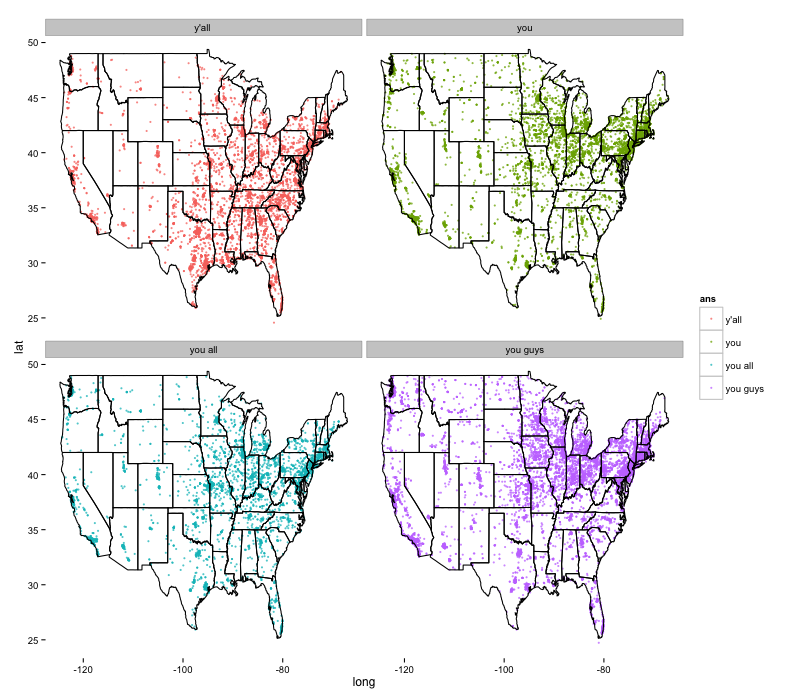
\includegraphics[width=400pts, height=250pts]{you_facet.png}
\caption{faceted plot for question 50: "What word(s) do you use to address a group of two or more people?"}

\end{figure}

I first inspected the plots on the website and picked a question that offered the most drastic difference in at least two responses as reflected in the geographic location. For instance, question 50, asking for what plural form of  `you' is used, offered one of the more distinct scatterplots to demarcate a north versus south trend, as we can see in the faceted plot above, especially between ``y'all"(red)  and the other three responses.  


\begin{figure}[H]
\begin{minipage}{.30\textwidth}
\vspace{7pts}
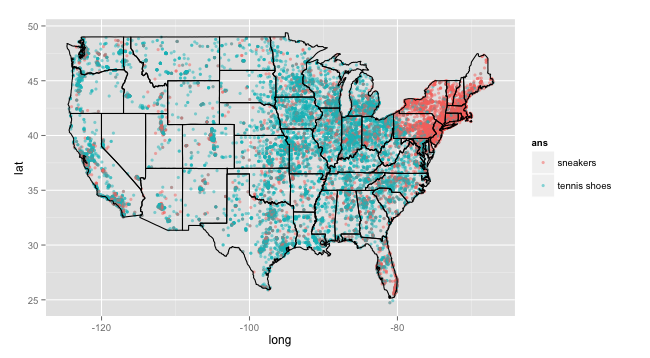
\includegraphics[width=220pts, height=125pts]{shoes.png}
\caption{Question 70: "What do you call gym shoes"}
\end{minipage}
\begin{minipage}{.60\textwidth}
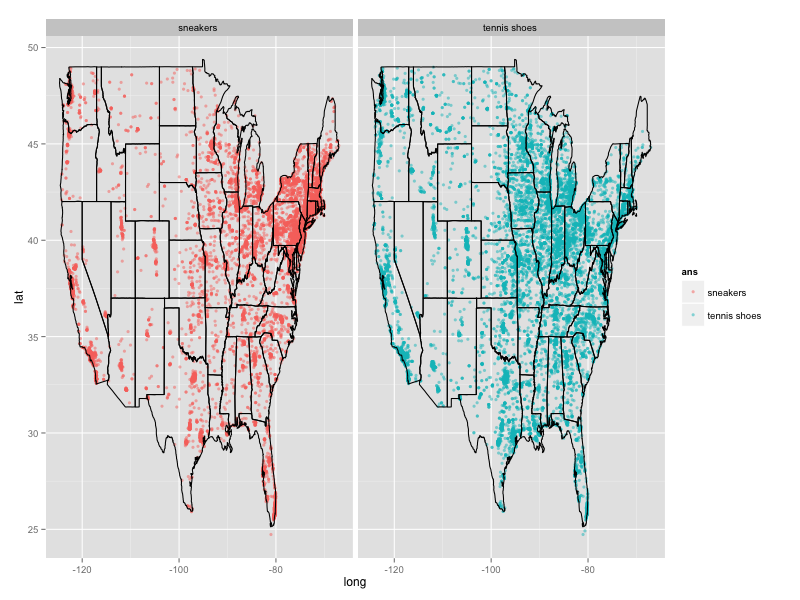
\includegraphics[width=400pts, height=120pts]{shoes_facet.png}
\vspace{-10pts}
\caption{Faceted plot for question 70}
\end{minipage}
\end{figure}

Question 73 was an example of one where two responses dominated the observations, and gave partially overlapping regions, with a noticeable symmetric difference.  The question asked what one calls gym shoes. The red points represented individuals who called them``sneakers", and blue represent the ``tennis shoes" response.  Without the facetted graph, the plot can look deceptively like it has drawn a strict border in the northeast (even with use of alpha and smaller point size).  But as we learn from the faceted plots, there is a much smoother transition, or rather, there is a gradual overlap.  This motivates reflecting on what it means to be a 'linguistic border'.  We certainly should not expect very discontinuous borders where linguistic patterns suddenly change, so when looking at clusters later in the analysis, there is a motivation to accept overlapping clusters, as linguistic transitions are gradual, and regions can be identified when one feature becomes dominant as another recedes.  

\begin{figure}[H]
\centering
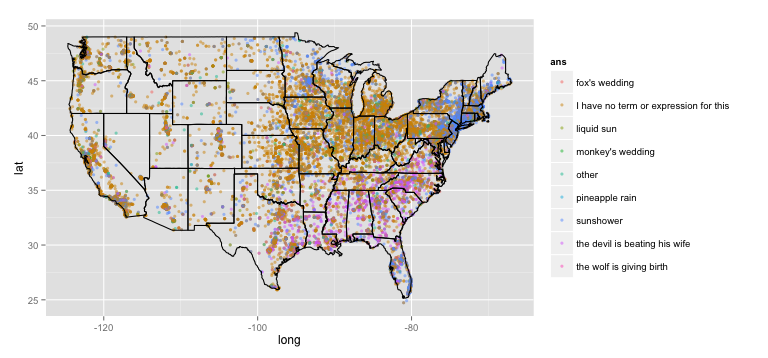
\includegraphics[width=450pts, height=200pts]{sunshower.png}
\caption{Scatterplot for question 80: "What do you call it when it rains and it is sunny?"}

\end{figure}

Finally, we offer question 80 as an example where interesting intersection patterns are found, but it is not obvious what regions they are revealing.  As we can see by the facetted plot, much of the geographic location of those who responded overlaps.  The smaller frequency responses also seem noisy. 


\begin{figure}[H]
\centering
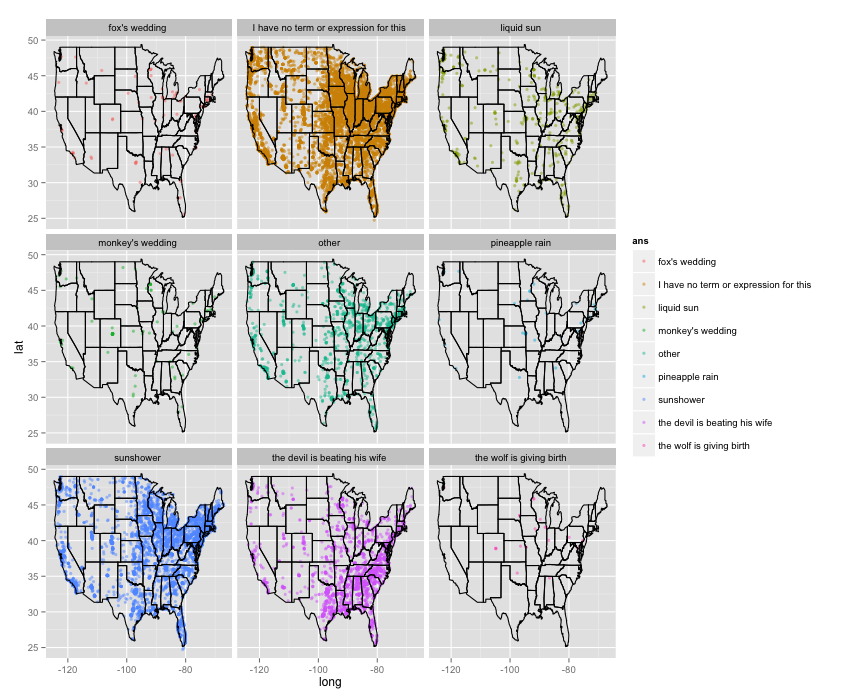
\includegraphics[width=550pts, height=300pts]{sunshower_facet.png}
\caption{faceted plot for question 80: "What do you call it when it rains and it is sunny?"}

\end{figure}


The aforementioned three questions offered little information about the relation between responses and regions.  As a check against dimension reduction techniques in the next chapter, I used just these three questions, in binary vector form, followed by kmeans clustering to see what kind of groups can be gleaned from the combined information of all three questions.  I experimented with 4,7,9 and 11 clusters, mainly chosen because beyond 11 there seemed to be too much noise and under 4 too much information was lost. I only plotted the facetted scatterplots for 4 and 9 here in the interest of space.  7 and 11 don't fit well in a square, and more importantly than aesthetic objections, they don't reveal much more.  The clusters in general in this exploratory trial are not very good, and the next section we will see much improvement.  I should note that using L1 did not improve the situation, even though it makes more sense to use L1 penalty for count data.  But we should not be surprised as the three questions were chosen rather arbitrarily.

\begin{figure}[H]
\centering
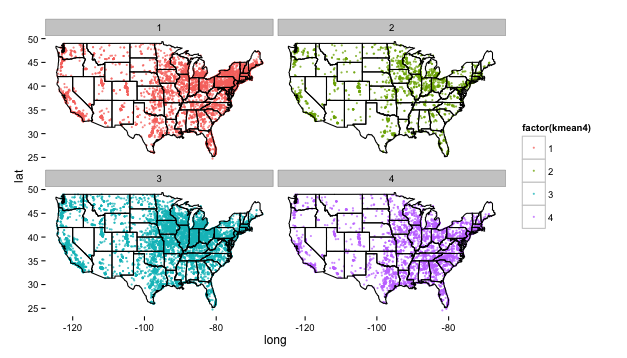
\includegraphics[width=300pts, height=180pts]{kmean4_dumb.png}
\caption{K means 4 clusters}
\end{figure}

\begin{figure}[H]
\centering
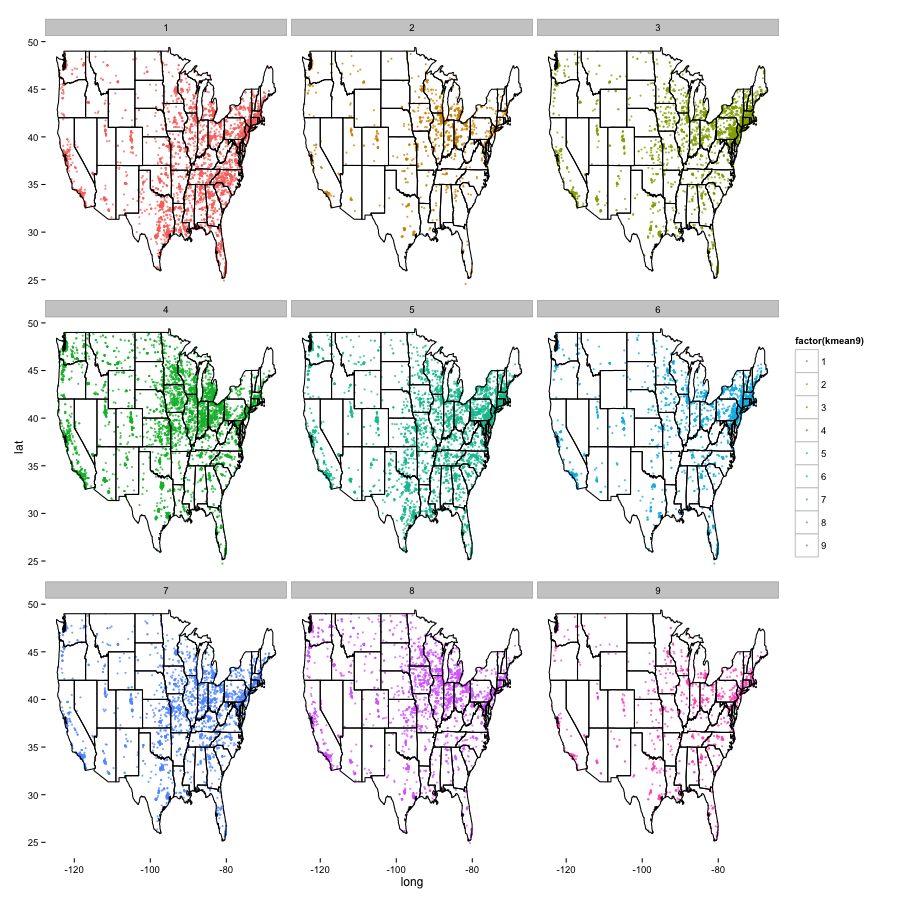
\includegraphics[width=400pts, height=240pts]{kmean9_dumb.png}
\caption{K means 9 clusters}
\end{figure}

\section{Dimension reduction methods}

Let's first establish a list of names for the datasets analyzed.\footnote{ Unfortunately I did not have time to standardize these names in the code files.  }
\begin{itemize}
\item {\bf Bin47471} Original linguistic data set with 47471 rows of observations converted to binary form.{\bf Bin.85} is the result of doing PCA and then projecting onto the subspace spanned by the first $k$ principle components that explains 85\% of the variance.  {\bf Bin.95} is the same as above only we project down onto more principle components to explain 95\% of the variance.
\item {\bf Lat.Long.Bin} Starting from the lingLocation dataset, which was provided, and already binarized and aggregated within the groups of 1 degree longitude-latitude squares (that is, the row information was simply summed per group). 
\item {\bf Lat.Long.Bin+Norm} Lat.Long.Bin with each row divided by the number of people in each group (i.e per latitude-longitude degree square).  This provided a rate of answers per group. {\bf Lat.Long.Bin.85} is the result of doing PCA and then projecting onto the subspace spanned by the first $k$ principle components that explains 85\% of the variance.  {\bf Lat.Long.Bin.95} is the same as above only we project down onto more principle components to explain 95\% of the variance.   
\item State were also used as a group, but no extra information was gained, if not too much lost, compared to the more finely aggregated datasets above, so we eliminate it from this write to save space.  
\end{itemize}


An important remark of justification: the normalized responses per grouped region can be interpreted as a probability to give a particular response, indexed by region.  For instance, a column vector of values under question 50 response``ya'll" gives a rate of response for each region the dataset is group by.   This interpretation aligns with viewing a person's response as the random variable, and thus each rate per region is a propensity to use language in a certain way, calculated by averaging the people's responses per region.  It's reasonable to regard responses are random variables because we are treating various factors of a person's life as the source of randomness that generates their speaking behaviour.  Assuming that these speaking patterns have finite and comparable variance (reasonable to assume since most of us need to communicate to function) highly dense areas will have rates that are normally distributed around their true mean, true propensity for the area (we have central limit theorem behaviour here because the empirical mean we calculate is normally distributed on this assumed true mean).  This interpretation of the data also helps us access why L2 penalty performed well on the aggregated datasets when initially we expected L1 to.  \\

We used PCA for dimension reduction on all the aforementioned datasets.  It was especially necessary for Bin.47471.  And they performed well as expected, since binarizing the datasets made the same information live in a higher dimensional space, and thus become more sparse (I am slightly simplifying since the original lower dimensional space is not a subspace of the higher dimensional one, but it is the right intuition for why PCA would perform well).  Of the 468 dimensions, only a 161-dim subspace was needed to account for 95\% of the variance, and 85 needed for 85\% (coincidence) for Bin47471.  I used the first 85, and 161 principle components, respectively, to span the subspace upon which the 468 dimensions of information were projected (dot product each principal component with every row of data to get a new 47471 $\times$ 85 and 47471 $\times$ 161 data frame).  These new data frames are now difficult to interpret, as column $k$ row $l$ represents how much of component $k$ person $l$'s data consists of.  But principle component $k$ is itself a linear combination of the 468 answers.  Inspecting the coordinates of the first couple of components (and arranging the coordinates in decreasing order by absolute value) I noticed that these values decrease almost linearly, and in particular, there is no noticeable cutoff, so we cannot attribute a large portion of the variance to a small  handful of question responses  This is not necessarily surprising, as how the 122 were chosen by the scientists is not clear, there may not have been strong reason to believe these are the most polarizing questions.  More importantly, all that the PCA reveals is that there is not one or two questions of particular importance, but certain decently sized (more than a couple) subsets are of particular importance, to explain the variation in responses.  \\

PCA on Lat.Long.Bin+Norm required 65 components to explain 95\% of the variance.  I also did the same analysis for 85\% of the variance, which did not make the k-means noticeably faster (both were very fast) and the plots were very similar.  So at least this offered a robustness check.  After performing PCA and projecting for Bin.47471 and Lat.Long.Bin+Norm, I experimented with kmeans and pam (partitioning around metroids), using both L1 and L2 penalty to cluster the datasets.  L1 made the most sense for the unaggregated Bin.47471 dataset, since it was the original count data.  We unfortunately could not get the algorithm to run without crashing using L1 penalty, so can only provide clustering data with L2 penalty for the Bin.47471 dataset.\\

 We experimented with 4-11 clusters for each dataset, and found Lat.Long.Bin+Norm revealed interesting information for even 11 clusters.  While that Bin.474741's clusters' useful information capped at 7 clusters.  By 7 clusters, New York began to emerge as region distinct from its surrounding areas, and Miami could already be identified as more similar to the Northeast rather than the rest of the south states.  New York at the 7 cluster point in the Lat.Long.Bin+Norm dataset was never really demarcated, perhaps more so by the 11 cluster point.  An interesting explanation for this is that Bin.47471, by using the raw count data per person, equally weighed each person as a random variable to generate the data.  Thus, clustering was sensitive to denser populations such as the New York areas.  But this information was averaged out and weighed less in the Lat.Long.Bin+Norm and County.Bin+Norm datasets, since each region was weighed the same.  This is why we could begin to see Texas by 9 clusters using L1 on Lat.Long.Bin and by 11 clusters using L2, yet it never shows up in the clustered Bin.47471 dataset, overshadowed by the more densely populated northeast, which is what began to fragment in the larger cluster graphs instead.  

\begin{figure}[H]

\begin{minipage}{.5\textwidth}
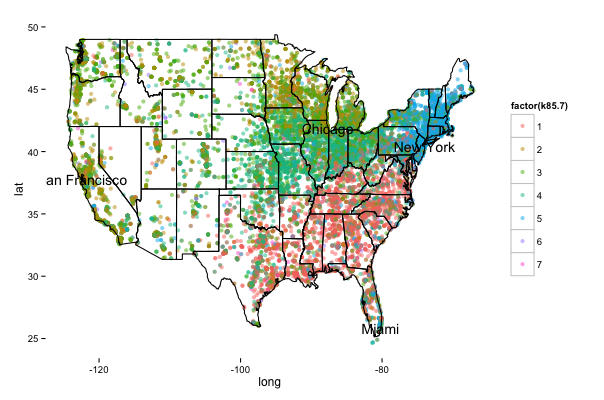
\includegraphics[width=250pts, height=150pts]{85_7.png}
\caption{kmeans-L2-85 variance PCA-7 clusters}
\end{minipage}
\begin{minipage}{.5\textwidth}
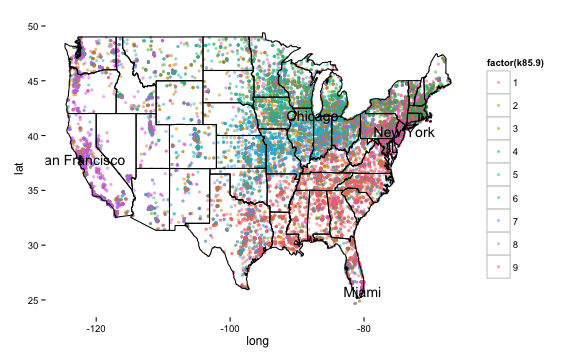
\includegraphics[width = 250pts, height=150pts]{85_9.png}
\caption{kmeans-L2-85 variance PCA-9 clusters}
\end{minipage}
\end{figure}

\begin{figure}
\begin{minipage}{.5\textwidth}
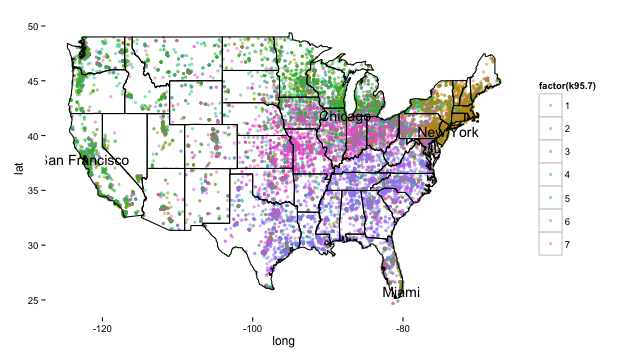
\includegraphics[width=250pts, height=150pts]{95_7.png}
\caption{kmeans-L2-95 variance PCA-7 clusters}
\end{minipage}
\begin{minipage}{.5\textwidth}
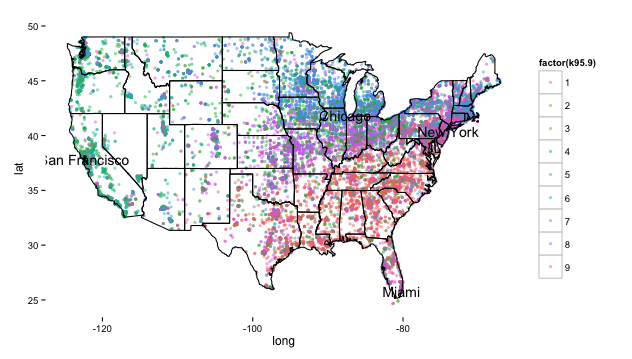
\includegraphics[width=250pts, height=150pts]{95_9.png}
\caption{kmeans-L2-95 variance PCA-9 clusters}
\end{minipage}

\end{figure}


As we can see, not much extra information was gained by using the 95 variance plot, and we confirmed this in more detail by comparing the set of facetted plots (so each cluster was plotted alone and compared across the 85, 95 datasets). Using 85\% of the variance was sufficient, which meant clustering on only 85 columns (a happy coincidence that 85 principle components was needed for 85\% variance).  by the time we got to 11 clusters for the 85 dataset, there as barely any geographic information detected.  In fact, the 7 clustered graph seems to carry as much information as the 9 cluster one.  It is interesting to note that when one zoom in near Miami, one can see that it is given the same combination of colours a those from the Northeast. This can be treated as a fuzzy classification of sorts, since belong to the same combination of clusters is also information to classify one as speaking very similarly, as we see in the case of Miami. \\

The faceted graph below for the 7 clustered dataset shows us exactly where the 7 clusters fall, as we can see, a couple of regions mostly did not intersect.  But some sparser clusters did.  Nonetheless, the overall effect when plotted together, as shown in figure 8's 5 distinct regions (as indicated by overall colour of the region).  This nicely aligns conceptually with the idea that a dialect is characterized by it's similarities as well as differences from other dialects.  So for instance, a Southern dialect can be identified by what it shares with all eastern regions, as well as by what it does not share with predominantly northeast and northwest $\cup$ west coast traits.  Again, categorizing dialects not strictly by a single membership in a cluster, but by how many cluster memberships it shares with other regions. \\
\begin{figure}[H]

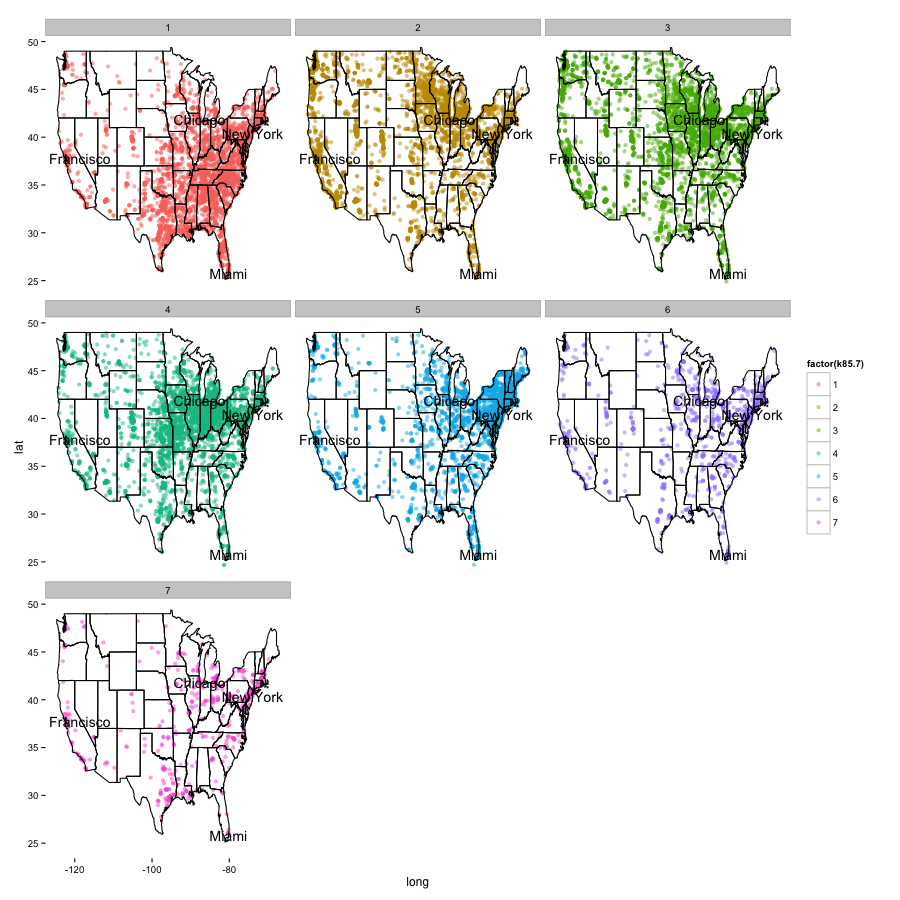
\includegraphics[width=550pt, height=380pts]{Rplot01.png}
\caption{Faceted 7 clusters from 85 variance dataset}

\end{figure}

The second set of most interesting finding came from clustering the Lat.Long.Bin+Norm dataset.   Here, we were able to successfully implement pam with L1 penalty, and it actually generated clusters different from L2, though both had their shining points.  It was also interesting to see what information was gained from the aggregation of data per unit latitude longitude area, and what information was lost.  We discuss below. 

\begin{figure}[H]

\begin{minipage}{.5\textwidth}
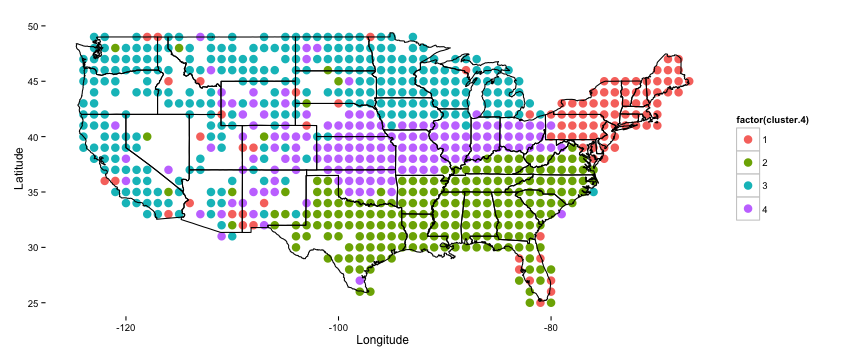
\includegraphics[width=250pts, height=150pts]{4clustersmall.png}
\caption{k means L2: 4 clusters}
\end{minipage}
\begin{minipage}{.5\textwidth}
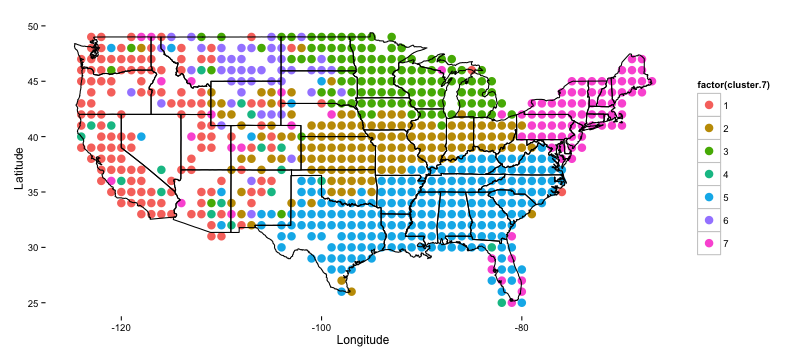
\includegraphics[width = 250pts, height=150pts]{7clustersmall.png}
\caption{k means L2: 7 clusters}
\end{minipage}
\end{figure}

\begin{figure}[H]
\begin{minipage}{.5\textwidth}
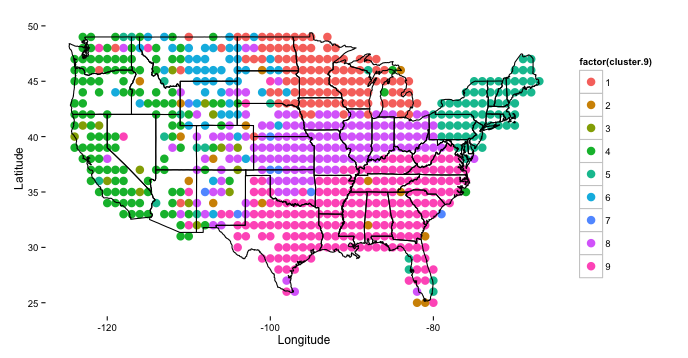
\includegraphics[width=250pts, height=150pts]{9clustersmall.png}
\caption{k means L2: 9 clusters}
\end{minipage}
\begin{minipage}{.5\textwidth}
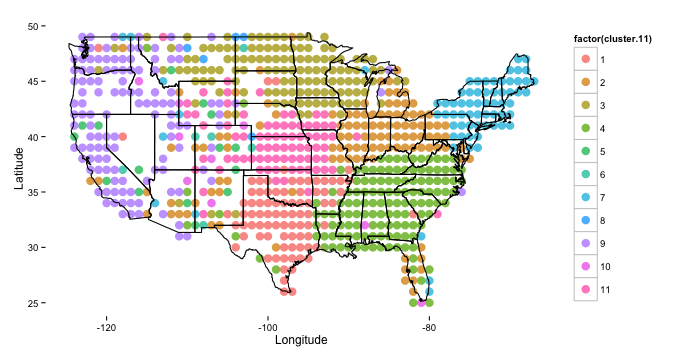
\includegraphics[width=250pts, height=150pts]{11clustersmall.png}
\caption{k means L2: 11 clusters}
\end{minipage}

\end{figure}

The aggregated dataset did very well considering how much smaller it is, compared to the to Bin.47471 dataset.  Algortihims for clustering took less than 2 seconds rather than minutes for Bin.47471. Below we used the pam algorithm (portioning around metriods) with L1 penalty. Kmeans was also used with both L1 and L2 penalty, and results were not too different across all methods.  We offer the plots of the three (kmeans with L2 penalty, kmeans with L1 and pam with L1 penalty).  Comparing the clusters of all three is a great validation of the clusters identified.  Even though more distinct regions were identified at the 11 cluster point by kmeans (L2) and pam(L1), the common borders between all three methods is a signal for the robustness of these clusters.  

\begin{figure}[H]
\begin{minipage}{.5\textwidth}
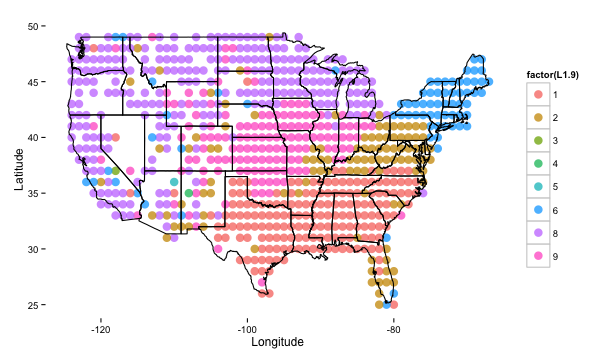
\includegraphics[width=250pts, height=150pts]{L1_9.png}
\caption{k means L1: 9 clusters}
\end{minipage}
\begin{minipage}{.5\textwidth}
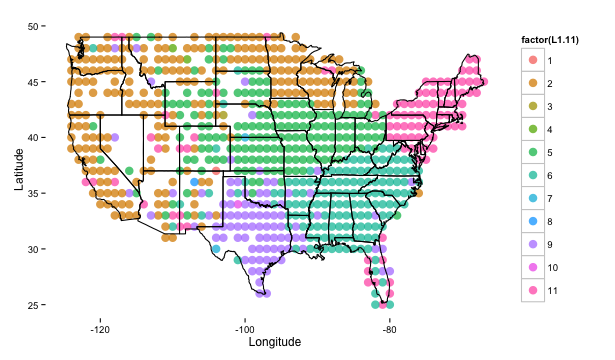
\includegraphics[width=250pts, height=150pts]{L1_11.png}
\caption{k means L1: 11 clusters}
\end{minipage}

\end{figure}

\begin{figure}[H]
\begin{minipage}{.5\textwidth}
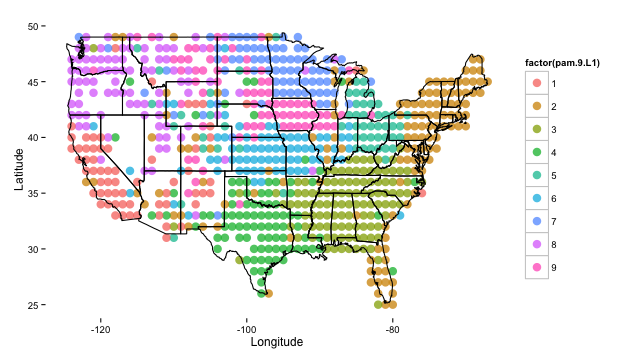
\includegraphics[width=250pts, height=150pts]{pam9.png}
\caption{pam L1: 9 clusters}
\end{minipage}
\begin{minipage}{.5\textwidth}
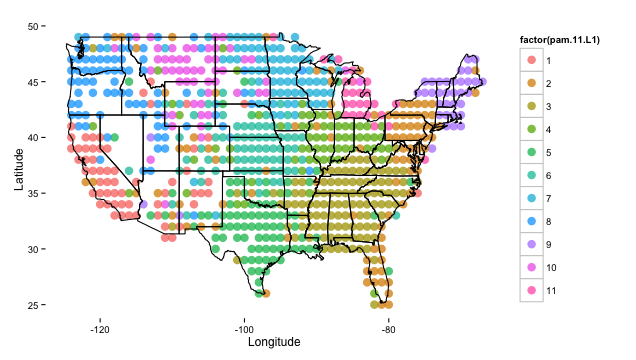
\includegraphics[width=250pts, height=150pts]{pam11.png}
\caption{pam L1: 11 clusters}
\end{minipage}

\end{figure}

Both L1 and L2 penalty for 11 clusters still managed to pick up more information than the 9 clusters.  There is no further need for faceted graphs since the data points do not overlap.  This observation also explains why the Lat.Long.Bin+Norm dataset produced more distinct clusters by region, compared to the Bin.47471 dataset. Nonetheless, not having overlapping points does not force the clusters to be connected regions, but we see that they are, and read it as evidence of the continuity of dialect patterns across geography.  We are also happy to note that Miami emerged in the same cluster as certain Northeast regions, so not all clustering can be explained by geographic proximity.  The case of Miami is robust across the two datasets and various clustering methods and metric penalties.  It is also not surprising, as Miami is a popular vacation destination to escape the harsh northeastern winters.  Being a cosmopolitan city, it attracts in general more standardized ways of speaking that is found in other metropolitan centers.  \\




\section{Stability of findings to perturbation}

The conclusions from Bin.47471 were very stable under removal of 20\% subsets of the dataset.  However, sampling out of the Lat.Long.Bin+Norm affected the clusters a bit more.  This is because certain points contain a lot more aggregated information than others.  As discussed previous, since high density regions presented the aggregated behaviour of many more people.  So I sampled before aggregating the data by the groupings, that is, from the 47471 dataset, and with this more fair sampling method, the clusters were mainly stable (borders were not exact, but the way the clusters picked out certain regions was robust) and even Miami remained stably part of the Northeast cluster.  Happily, points up in Washington state identified as part of the texas cluster sometimes disappeared (figure 18), validating the fact that those were noise.  This is also confirmed by the fact that none of the other plots found displayed this phenomenon.\\

It is not clear which of the L1 or L2 methods performed better.  Both identified similar clusters, including identifying San francisco by 11 clusters with L2, and by 9 clusters with L1.  San francisco is shown as in the same cluster as the new york area in both methods, so can be treated as a robust finding like Miami.  \\


 An extension of the work done in this lab would be to use the cluster information to come up with a predictive model for identifying where a person is from just by using their answers to the survey.  Regrettably there was no time to complete this.  

I should mention that centering and not centering the dataset made very little difference in number of components needed, and it made less sense to center (there is no reason why we expect each question response to have on average 0 responses) so I stuck with the uncentered dataframes for analysis to make the results more interpretable.  \\

Initially I wanted to try hierarchical clustering since it makes more sense to define a similarity rather than the more restrictive distance metric between data points. Yet it was difficult to get the algorithms not to crash.  This is thus an area for further exploration in the lab.  

\section{Conclusion and Extensions}

The linguistics survey dataset revealed a surprising amount of information about the geographic borders of dialect differences.  It demonstrated the successful use of PCA to concentrate on a lower-dimensional subspace of data where most of the variation in observations take place (and thus also helps ignore noise), and robust cluster findings using different penalties and aggregations of the dataset.  Some room for further investigation is to employ non-distance based clustering methods, and also to build predictive models based on the learned clusters to further validate the clusters generated.  The interpretability of the subspace given by the PCA can also be examined in more detail to help weigh the more useful/polarizing questions in the survey.  


\section{Appendix}

Below we first use a normal kernel smoother for each node and also one for the aggregate data. 
\begin{figure}[H]
\begin{minipage}{.5\textwidth}
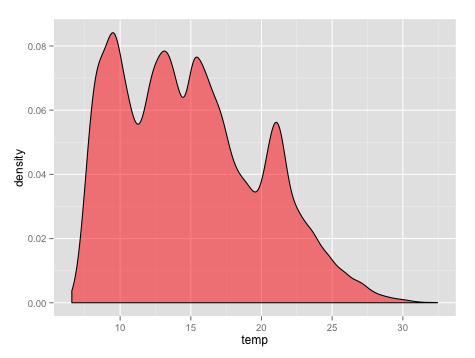
\includegraphics[width=250pts, height=150pts]{Rplot02.png}
\caption{normal density for mote higher than 45 meters}
\end{minipage}
\begin{minipage}{.5\textwidth}
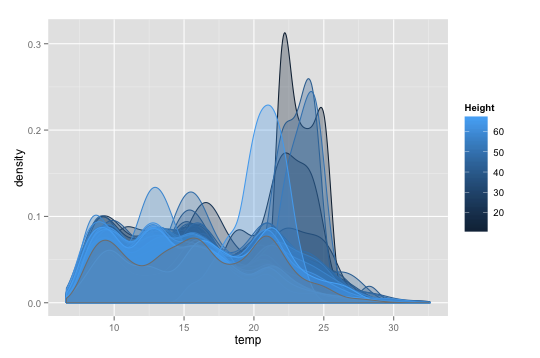
\includegraphics[width=250pts, height=150pts]{height_density.png}
\caption{kernel smoothers for various heights (as factor)}
\end{minipage}

\end{figure}

A Loess smoother of degree 1 was enough to capture most of this information.  

\begin{figure}[H]
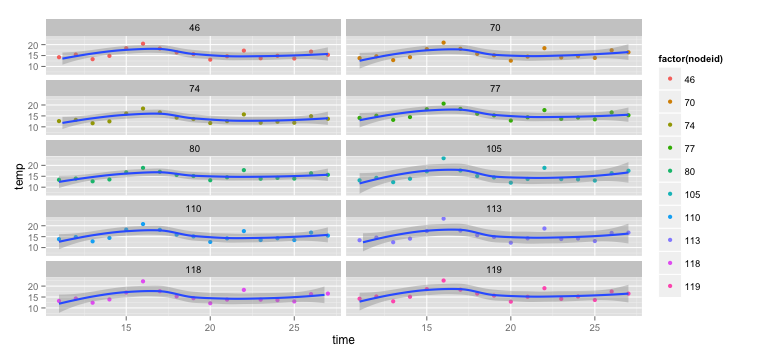
\includegraphics[width=400pts, height=400pts]{loess_smooth.png}
\caption{Loess Smooth by nodes of similar height}


\end{figure}

\end{document}